%-----------------------------------------------------------------------------
%
%               Template for sigplanconf LaTeX Class
%
% Name:         sigplanconf-template.tex
%
% Purpose:      A template for sigplanconf.cls, which is a LaTeX 2e class
%               file for SIGPLAN conference proceedings.
%
% Author:       Paul C. Anagnostopoulos
%               Windfall Software
%               978 371-2316
%               paul@windfall.com
%
% Created:      15 February 2005
%
%-----------------------------------------------------------------------------


\documentclass[10pt, preprint]{sigplanconf}

% The following \documentclass options may be useful:
%
% 10pt          To set in 10-point type instead of 9-point.
% 11pt          To set in 11-point type instead of 9-point.
% authoryear    To obtain author/year citation style instead of numeric.

\usepackage{amsmath}
\usepackage{graphicx}
\usepackage{subfigure}
\usepackage{multirow}
\usepackage{rotating}
\usepackage{array}
\usepackage{algorithmic}
\usepackage{algorithm}
\usepackage{textcomp}
\usepackage{listings}
\usepackage{hyperref}
%\usepackage{cite} %after hyperref

\begin{document}

\conferenceinfo{WXYZ '05}{date, City.} 
\copyrightyear{2011} 
\copyrightdata{[to be supplied]} 

\titlebanner{preprint}        % These are ignored unless
\preprintfooter{Naming Anonymous JavaScript Functions}   % 'preprint' option specified.

%\title{Better JavaScript Runtime Understanding by Automated Function Name Extraction}
%\title{JavaScript Lost Names, Is There Any Solution?}
%\title{JavaScript Lost Names, Any Amendment?}
%\title{Fixing Lost JavaScript Function Names in Debuggers}
\title{Naming Anonymous JavaScript Functions}
%\subtitle{Subtitle Text, if any}

\authorinfo{Salman Mirghasemi}
           {\'Ecole Polytechnique F\'ed\'erale de Lausanne(EPFL)}
           {salman.mirghasemi@epfl.ch}
\authorinfo{John J. Barton}
           {IBM Research - Almaden}
           {bartonjj@us.ibm.com}
\authorinfo{Claude Petitpierre}
           {\'Ecole Polytechnique F\'ed\'erale de Lausanne(EPFL)}
           {claude.petitpierre@epfl.ch}

\maketitle

\begin{abstract}
Understanding JavaScript code due to its dynamic, weakly-typed nature is complicated. Developers usually comprehend JavaScript programs by running them and examining their elements at runtime. However, understanding concrete values, particularly user-defined and function objects, is not always straightforward. Function names can aid in this regard; they can appear as the constructor name in object representation or as the function identifier in call-stack. Based on our analysis over ten famous JavaScript projects, unfortunately only a very low proportion (less than 7\%) of JavaScript functions are named by developers in the first place. As a solution to this problem, we propose an automated approach based on local source code analysis for naming nameless JavaScript functions. We applied our approach on several JavaScript projects and the results are very promising.
\end{abstract}

\category{D.2.5}{Testing and Debugging}{Debugging aids}
\category{D.2.6}{Programming Environments}{Integrated environments}

\terms
Algorithms, Human Factors, Languages

\keywords
JavaScript, Function Name, Debugger

\section{Introduction}
The unique and important role of JavaScript in web programming is undeniable. Along with the wave of ``Web 2.0", JavaScript has become the inevitable part of almost every modern web site. This language is used by all of the web's 100 most popular sites\footnote[1]{http://www.alexa.com}. It is very likely that JavaScript keeps this crucial role for the next few years or even the next decade. Along with the growth of demands for more comprehensive user interfaces, the size and the complexity of web applications is increasing. Moreover, JavaScript is also becoming a general purpose computing platform with office applications \cite{JSOffice, JSOffice2}, browsers \cite{FAO, GCE} and development environments \cite{Ingalls} being developed in JavaScript \cite{Richards}. There are also proposals for employing JavaScript in server-side applications \cite{SSJSR, CJS}.

To cope with these large and sophisticated systems, JavaScript developers turn to better development tools. These tools analyze then represent the program in ways that the developer might only be able to imagine through substantial time-consuming reading of source code.  One prime example is a runtime debugger: the developer can halt a running program and examine the program state and execution call stack. All of these tools need to express program artifacts in a compact way the developer can understand.  For example, the debugger needs to present the execution call stack so the developer can understand which functions are currently active.  Obviously a particularly good compact representation would be a name given by the developer in the source code. However, the JavaScript language itself does not require names for many program artifacts and -- as we shall see -- nameless or anonymous artifacts are more common than named ones. Anonymous artifacts prevent tools from communicating effectively with developers.

Among program artifacts, functions are central to program comprehension in JavaScript. In addition to their role in the execution stack, they are first-class objects that are used for different purposes by developers; they may be used as an object constructor, a closure scope (module) or even  passed as an argument in a function call. However, functions can be defined and created without a name or identifier.  

In this paper, we analyze function creation and consumption in ten large, well-known projects. We show that within these projects less than 7\% of the function objects are named. We propose an automated approach based on extracted data from the source code for naming JavaScript functions. The candidate function names can be used in debuggers for more descriptive object summaries and call-stack view, or in integration with proposed JavaScript typing systems for providing modern editing features in development environments. 


%In this paper, we analyze function creation and consumption in ten famous project. We propose an automated approach based on extracted data from the source code for naming JavaScript functions. The candidate function names can be used in debuggers for more descriptive object summaries and call-stack view, or in integration with proposed JavaScript typing systems for providing modern editing features in development environments. 

%The function name is necessary for referring and recalling the function's functionality, but only a small proportion (less than 7\%) of JavaScript functions are named.



%\section{The Nameless Function Problem}
\section{The Anonymous Function Problem}

A JavaScript function can be defined with the {\small\texttt{function}} operator or the {\small\texttt{Function}} constructor (i.e., {\small\texttt{new Function(args, source)}}) \cite{ECMA}. The {\small\texttt{function}} operator can appear in a function declaration, function expression, or function statement (the latter form is available in Firefox but not part of a standard).  Of these forms, only the function declaration requires a function name and the {\small\texttt{Function}} constructor has no mechanism to name the function.  In other words, JavaScript developers can define functions with or without function names.

If you are unfamiliar with JavaScript or other functional programming languages, you might imagine that developers would naturally select the form with names, simply as an organizational tool. However this is not the case. Functions in JavaScript are first-class objects. They can be assigned to any variable or object property, or passed as an argument to a function. Consequently JavaScript programmers can use this constructs to organize their thinking about the program, without the use of function names.

So what do JavaScript developers do in practice?  To get empirical evidence we analyzed the source code of ten well-known JavaScript projects. For every project, the total number of functions and the number of functions with an identifier are collected (Table~\ref{js-functions}). The average ratio of named functions to all functions is less then 7 percent and excepting one project (Prototype), the ratio does not exceed 13 percent. Our analysis does not include the functions defined by dynamically created evaluated scripts created by {\small\texttt{eval}} function). Among all functions only a very limited number of them (116 functions) are defined by the {\small\texttt{Function}} constructor. Therefore, we conclude that a large proportion of JavaScript functions are anonymous.



\begin{table}
\centering
\scalebox{0.9}{
  \begin{tabular}{ | l | l | l | l | l |}
  \hline
   Project & Description & Total & Named \\ 
  \hline 
   Closure & Google Web Library & 9195 & 208(2\%) \\ 
  \hline 
   DoJo & JavaScript Toolkit & 18676 & 2810(15\%) \\ 
  \hline 
   ExtJS & JavaScript Framework & 37717 & 1184(3\%) \\ 
  \hline 
   Firebug & Web Development Tool & 3424 & 406(11\%) \\ 
  \hline 
   jQuery & JavaScript Library & 422 & 23(5\%) \\ 
  \hline 
   MochiKit &  JavaScript Library & 1866 & 37(1\%) \\ 
  \hline 
   MooTools & JavaScript Framework & 625 & 7(1\%) \\ 
  \hline 
   Prototype & JavaScript Framework & 645 & 203(31\%) \\ 
  \hline 
   Scriptaculous &  JavaScript Library & 1092 & 208(19\%) \\ 
  \hline 
   YUI &  Yahoo UI Library & 22346 & 922(4\%) \\ 
  \hline 
   All &  & 96008 & 6008(6.3\%) \\ 
  \hline 
  \end{tabular}
  }
\caption{The total number of functions and the number of named functions (and percent named)  in ten large JavaScript projects. See appendix 1 for the project citations.}
\label{js-functions} 
\end{table}    


\begin{figure}[htp]
%{\small 
%\begin{verbatim}

\lstset{basicstyle=\scriptsize}
\lstset{emph={FOO,BAR},emphstyle=\textit}
%\lstset{backgroundcolor=\color{yellow}}
\lstdefinelanguage{myLang}
{morekeywords={if, function, var, return, new}}

\begin{lstlisting}[frame=single, language=myLang]
9  var main = function() {         // main<
10   return function() {           // main
11     var foo = new FOO("a");
12     var bar = new BAR("b");
13     var result = op(
14       function(value){          // main/result<
15         return value;
16        });
17   }
18 }();
19 var FOO = function(a) {         // FOO
20   this.a = a;
21 }
22 var BAR = function(b) {         // BAR
23   this.b = b;
24 }
25 var op = function() {           // op<
26   var local;
27   return function(callBack) {   // op
28     local++;
29     return callBack(local);
30   }
31 }();
\end{lstlisting}
%\end{verbatim}}
\caption{An excerpt of a JavaScript code.}
\label{js-code}
\end{figure}


\begin{figure*}[htp]
\centerline{
\subfigure[Google Chrome Debugger]{\label{fig_object_second_case}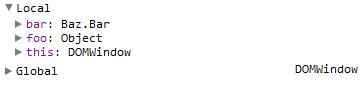
\includegraphics[width=0.47\textwidth,height=.15\textheight]{pic/chrome-objects.jpg}}
\hfil
\subfigure[Firebug]{\label{fig_object_first_case}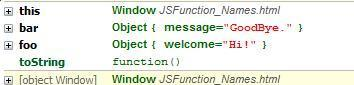
\includegraphics[width=.47\textwidth,height=.15\textheight]{pic/fbug-objects.jpg}}}
\caption{The screenshot of variables view of Google Chrome and Firebug JavaScript debuggers paused on a breakpoint at line 15 of the program shown in Figure~\ref{js-code}.}
\label{debuggers-objects}
\end{figure*}

To understand the consequences of anonymous functions on development tools we will focus on one example, the impact on debuggers.
Two main issues appear in debuggers due to the lack of function name. First, object constructor name, which can facilitate understanding the object value, is not available in the object summary. Second, the call-stack view is usually full of \textit{anonymous} functions and therefore much less informative. We discuss these issues in the next two subsections. 
 
\subsection{Missed Constructor Name in Object Summary}
JavaScript doesn't support classes, but objects can be created by constructors ({\small\texttt{new Constructor()}}). A constructor is a regular JavaScript function. Once the {\small\texttt{new}} keyword is evaluated, an empty object, with the constructor prototype as its prototype, is created, then the new object is bound to {\small\texttt{this}} and the constructor is called. The role of constructor is to initialize the empty object. Although the structure of object imposed by the constructor, unlike class-based object-oriented languages, may not remain intact during the object's lifetime \cite{Richards}, the constructor can still be used to classify the object. 
Debuggers employ this fact and display the constructor name in the object summary to facilitate developer's understanding. 

Figure~\ref{js-code} demonstrates an excerpt of a JavaScript code. We set a breakpoint on line 13 and examine the runtime elements at this breakpoint by two JavaScript debuggers, Google Chrome and Firebug (Figure~\ref{debuggers-objects}). Two objects assigned to variables {\small\texttt{foo}} and {\small\texttt{bar}} are constructed by two different constructors: {\small\texttt{FOO}} and {\small\texttt{BAR}}. However, Google Chrome debugger shows the general class of {\small\texttt{Object}} as the summary for both objects. The developer has to expand the object nodes to recognize their similarities and differences. Firebug classify objects in the same general class, but includes some of the object properties in the summary. These additional properties may hint the developer about the object structures. {\small\texttt{FOO}} and {\small\texttt{BAR}} definitions at lines 19 and 22 explain the debuggers' behavior; the function statements has no explicit name (identifier), therefore debuggers considered them as \textit{anonymous} functions.




\subsection{Anonymous Function Names in Callstack View}
To illustrate the second issue, we pause the program (Figure~\ref{js-code}) at line 15 by a breakpoint. Figure~\ref{debuggers-callstack} shows how the program call-stack is displayed in Google Chrome debugger and Firebug. The differences in the number of frames and line numbers between two call-stacks are due to dissimilar event handling implementations in the underlying platforms. Google chrome shows \textit{anonymous} as the name of all functions excepting the first one. Firebug performs better by guessing three function names but it still fails in one case. In these cases, the information provided by debugger is useless and the developer has to locate the function source to understand or recall the function behavior. 


\begin{figure*}[htp]
\centerline{
\subfigure[Google Chrome Debugger]{\label{fig_second_case}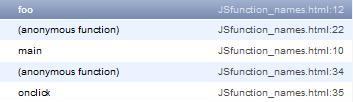
\includegraphics[width=0.47\textwidth,height=.13\textheight]{pic/chrome-callstack.jpg}}
\hfil
\subfigure[Firebug]{\label{fig_first_case}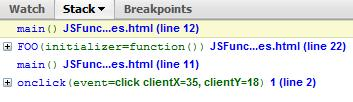
\includegraphics[width=.47\textwidth,height=.13\textheight]{pic/fbug-callstack.jpg}}}
\caption{The screenshot of call-stack view of Google Chrome and Firebug JavaScript debuggers paused on a breakpoint at line 15 of the program shown in Figure~\ref{js-code}.}
\label{debuggers-callstack}
\end{figure*}
 
Two other pieces of information which are important at function calls are {\small\texttt{this}} and argument values. In JavaScript, {\small\texttt{this}} like arguments is not defined by lexical scopes but it is bound once the function is called. The {\small\texttt{this}} value is missed in both views. The {\small\texttt{arguments}} values is shown in Firebug, but it still suffers from the same issues as object summaries.

\section{Automated Function Naming}
The anonymous functions problem is discussed in several articles and forums on the web \cite{DisplayName, Zaytsev}. Different solutions have been proposed and discussed by practitioners. A basic solution is a mechanism for naming functions by developers without affecting the variables in scopes. For example, a new property (e.g., \textit{displayName}) in the function object can be used for storing the function name, or the function name can be defined by an annotation. Although these solutions may help, they cause developers extra work, the annotation may be incorrectly recognized in programs that use the same property name for another purpose, and maintenance of the debugger becomes more difficult once the call-stack names can be overridden by user code.

We instead propose an almost automated approach for naming all functions by analyzing the source code. Before getting into explaining the algorithm details we discuss the rationale behind some of decisions we made in this approach.

\subsection{What Should Be Named?}

Once a statement which defines a function is evaluated, a new {\small\texttt{Function}} 
object is created.  The definition may be evaluated multiple times, and depending on the times a function definition is evaluated, 
zero to many {\small\texttt{Function}} objects can be created from the same definition. 
Two function objects which are created from the same function body may have different object properties added at runtime. They also may have different enclosing scopes and therefore different behaviors.  Thus our first 
decision: do we try to name the {\small\texttt{Function}} objects or the source that defines them?

For the common use cases, the different {\small\texttt{Function}} objects are bound to one or more properties of objects. The  names of these properties inform the developer about the role of the function in the actions of the object.  To determine the actions of the functions in turn, the developer must read the function source (or perhaps its documentation). Our function names serve to recall or summarize that source or documentation for the developer. Therefore we seek to name the source, the content between the curly braces known as the {\textit{FunctionBody}} in the standard\cite{ECMA}.

After reflection the reader may be puzzled by the preceding claim. On the one hand we claim that the function object instance may be bound to properties in multiple objects and those property names are not helpful for naming. On the other hand we will shortly introduce an algorithm that uses a property name (in part) to name a {\textit{FunctionBody}}. Ultimately we are relying on a subtle characteristic of JavaScript programming: the first binding of a {\textit{Function}}  to an object property differs from all other bindings because it is located in text near the {\textit{FunctionBody}} and thus developers associate this first binding with the meaning of the {\textit{FunctionBody}}. 

\subsection{What Makes a Good Function Name?}
A function name is basically used to assist the developer to recall or understand the function behavior. For a developer who is already familiar with the function, it works more like an identifier. However, this identifier should be easily recognized by the developer. For example, a naive proposal for the function name is a combination of the function file name and its first line number. Although it may work as an identifier, but it does not assist the developer to recall or understand the function behavior.

 On the other hand, for a developer who does not know the function, a function name should explains the function behavior, or an abstraction of the function behavior, or why/where the function is used/defined (e.g., to create the object \textit{foo}). A function name must not be too long that can not be displayed or read by the developer. For example, the function body explains the function behavior well however it is not an appropriate function name.

\subsection{Context, Package and Function Names}
JavaScript does not support a standard packaging mechanism to be used for modular programming. Scripts are loaded from different files and executed within the same or different global objects. Developers usually use objects at the top level to encapsulate properties, objects and functions from a framework or library. The same mechanism is reused for defining subpackages. As the project size and the number of functions increases, the short function name will not be enough for recognizing the function. The developer also wants the class or the module contains the function. In addition to the package name, knowing the context (the enclosing function body) that contains the function can help in better understanding the function behavior.

%\subsection{Is it possible to automatically name functions?}
%\subsubsection{Static vs. Dynamic}
% Can we improve the names at runtime?
% function object path in dom model is good candidate for the name but only for persistent objects ?

%\subsubsection{Local vs. Global}
%the object bound to {\small\texttt{this}}-depending on the way the function is called-and passed arguments. The first two parameters can be almost known from the source code and are less dependent to the runtime while the last two parameters are usually not known until the function call at runtime. 

%\subsubsection{Is it possible to automatically name all functions?}

%\subsubsection{Other Challenges}%
% functions pass the name as string, different types of class definitions

\section{Static  Function Object Consumption}

We call our automated naming solution "Static Function Object Consumption", since it relies only on a parser (static) and it attempts to name function bodies by tracking the function object created from the body to where the object is 'consumed', for example by binding to an object property, variable reference, or function argument.
Static Function Object Consumption generalizes the built-in JavaScript naming and common, simple coding patterns like object property initializers and variable assignments typically recognized by developers as naming functions.
The built-in naming, a function declaration, binds a name in a scope to a function object created from the adjacent function body. For example, in  {\small\texttt{function foo() \{return 1;\}}}, the name  {\small\texttt{foo}} is bound the the function body in curly braces.
Object property initializers bind a object property name to a function created from an adjacent function body. For example,  {\small\texttt{var bar = \{foo: function()\{return 2; \}\}}}, sets {\small\texttt{bar.foo}} to a function object created from the body {\small\texttt{\{return 2;\}}}. While the language does not associate the function body with the property  {\small\texttt{bar.foo}}, a JavaScript developer would because the created function body initializes the property. Similarly, a varible name bound to a function object, such as {\small\texttt{var baz = function()\{return 3; \}}}, is naturally associated with the function body. All three of these simple cases share the character that a function body creates a function object which is then bound to an identifier. 

Our algorithm applies the same logic: we follow the function object backwards through the code to create a name in cases where an identifier is not directly given in the code.
By 'backwards through the code' we mean that we parse the JavaScript and analyze the resulting syntax tree. For each function body, we walk up the tree looking for the constructs in table 2. As we describe in section XX, for every matching construct we record identifiers or expressions to use in constructing a name. 
Then we assemble a name using the expression-reduction rules outlined in section YY and the context naming rules in section ZZ. The result is a summary that contains identifiers (i.e., variable and property names) and strings available in the source code plus some explanatory tokens. It compactly explains the function object creation, consumption and assignment. For the simple cases of function declaration, object property initialization, and variable initialization the algorithm gives the same results we described above.

%	We instead, to tackle the aforementioned issues caused due to the lack of function names, propose automated function naming by anlyzing the source code. Before getting into details of how the function name is constructed, we discuss the rationale behind some of decisions we made in this approach.
%  Developers usually understand and refer to function objects by aliases they use to access them. This fact particularly holds for permanent function objects such as classes and utility functions. However, functions with shorter lifetimes such as closures and callbacks are referred by their roles or purposes in the program. We employ these facts to construct an identifier for a function. We analyze the source code and build a summary that explains the function object creation, consumption and assignment.
This summary which only contains identifiers (i.e., variable and property names) and strings available in the source code gives us the ingeredients for function identifier construction.
  
  %We analyze the source code to obtain the alias(es) that used for the function object or  is assigned to. If the list of aliases is not empty we select the most appropriate one based on some ranking rules as the function name. Otherwise, we try to build a name based on the aliases that the function object somehow affect on their values. If there is no such alias then the function object is consumed as an argument in a chain of function calls that does not return any value or as a simple closure. In the case of function calls chain we use the most nested called function name for constructing the identifier. In the case of simple closure, we employ the function(s) identifier inside the closure to construct the identifier. 
  
  
    %  On the other hand, it is very likely that the function object is assigned to this name in a place very close to the place the function object is created. Therefore, we analyze the code to find all names that the function object is assigned to them. For cases where the function object is not assigned to a variable or object property but is used to produce other values we keep track of the function effect on other identifiers.
      
\subsection{Example}
  
To illustrate the basic idea, we use the JavaScript code presented in Figure~\ref{js-code}. We can recognize seven function bodies in the code, none of them has a name. 

The first function on line 9 is called just after its creation (see line 18) and the return sets the {\small\texttt{main}} value. We can explain the function object consumption after its creation in two steps: 1) the function object is called (case 9 in table 2). 2) the result is assigned to {\small\texttt{main}} (case 6 in table 2). This differs from the simple variable assignment case: the value of {\small\texttt{main}} is not a function object but rather the return value of a function object.   We summarize this by saying that the result object is produced by the function object or the function object contributed to the {\small\texttt{main}} value and we write it {\small\texttt{main<}}, where the symbol {\small\texttt{<}} indicates "contributes to".

The function in line 10 is returned just after its creation. However, as the enclosing function is just called after its creation we can follow the function object flow in the enclosing scope and see that the function object is assigned to {\small\texttt{main}}. The summary of the function object consumption will be: 1) the function object is returned (case 10, table 2), 2) the function object is assigned to {\small\texttt{main}} (case 6 table 2). As the function object is directly assigned to this variable we name the function {\small\texttt{main}}. BUT I DON"T GET IT.
   
The third function, line 14, is passed to a function {\small\texttt{op}} on line 13, within the body of the function we named {\small\texttt{main}} . Here 1) the function object is passed as an argument to function {\small\texttt{op}} (case 11), 2) The call result is assigned to {\small\texttt{result}} (case 6). If we simply put of identifiers in this summary together we get {\small\texttt{main/result<op()}}. The first part before slash  shows the context name (the enclosing function name) for this function.  However, the function names (here {\small\texttt{op()}}) usually give an indirect information (e.g., role) about the function object. Therefore, as we explain in the next subsection, we ignore them if other kind of identifiers (e.g., variable and property name) are available in the summary. After dropping {\small\texttt{op}}, we will have {\small\texttt{main/result<}}. Eliding identifiers is important to avoid creating long, unwieldy names.

The next two functions, {\small\texttt{FOO}} on line 19 and {\small\texttt{BAR}} on line 22 are simple examples of case 6.  The last two functions defined in lines 25 and 27, similar to functions in lines 9 and 10, are named {\small\texttt{op<}} and {\small\texttt{op}} respectively. 


\begin{table}
\centering
\scalebox{0.8}{
\renewcommand\arraystretch{2.0}
\begin{tabular}{ | c | l | l | l | m{2.5cm} | l|}
  \hline
   & \multicolumn{4} {| c |}{Description} & \multicolumn{1} {| c |}{Code} \\ 
  \hline 
   1 &
   & 
   &  
   & direct access.
   & bar\textsuperscript{*}.foo = function()\{...\}\\
   \cline{0-0}\cline{5-6} 

   2 & \multirow{11}{*}{\hspace{.2cm}\begin{rotate}{90}The function object is\end{rotate}} 
   & 
   & 
   & \raggedright hashmap access by a string. 
   & bar\textsuperscript{*}["foo"] = function()\{...\} \\
   \cline{0-0}\cline{5-6} 

   3 &
   & \multirow{8}{*}{\hspace{.2cm}\begin{rotate}{90}assigned to a(n)\end{rotate}}
   & \multirow{5}{*}{\hspace{.2cm}\begin{rotate}{90}object property through\end{rotate}}
   & \raggedright hashmap access by a variable name.
   & bar\textsuperscript{*}[foo] = function()\{...\} \\
   \cline{0-0}\cline{5-6} 

   4 &
   & 
   & 
   & \raggedright hashmap access by a JavaScript expression.
   & bar\textsuperscript{*}[foo\textsuperscript{*}] = function()\{...\} \\
   \cline{0-0}\cline{5-6} 
      
   5 &
   &
   &
   & \raggedright  array index.
   & foo\textsuperscript{*}[0] = function()\{...\} \\
   \cline{0-0}\cline{4-6} 

   6 &
   & 
   & \multicolumn{2}{|l|}{
      variable.}
   & foo = function()\{...\} \\
   \cline{0-0}\cline{4-6} 

   7 &
   &  
   & \multicolumn{2}{|m{2.8cm}|}{
     \raggedright property of a new object in an object literal.}
   & \{ ..., foo: function()\{...\}, ...\}\\ %{\small\begin{verbatim}{ ..., foo: function(){...}, ...}\end{verbatim}} \\ %
   \cline{0-0}\cline{4-6}
	 
	 8 &
	 & 
	 & \multicolumn{2}{|m{2.8cm}|}{
	   new array index in an array literal.} 
   & [..., function()\{...\}, ...] \\ 
   \cline{0-0}\cline{3-6} 

   9 &
   & \multicolumn{3}{|m{3.8cm}|}{
     \raggedright directly called.}
   & function()\{...\}() \\
   \cline{0-0}\cline{3-6} 

   10 &
   & \multicolumn{3}{|m{3.5cm}|}{
     \raggedright returned from a function call.}
   & \{... return function()\{...\}\} \\
   \cline{0-0}\cline{3-6} 

   11 &
   & \multicolumn{3}{|m{3.5cm}|}{
     \raggedright passed as an argument to a function.}
   & foo\textsuperscript{*}(..., function()\{\}, ...) \\
   \hline 

  \end{tabular}
  }
\caption{Different cases of function object creation and usage in JavaScript.}
\label{table:function-types} 
\end{table}

 
\subsection{Overview of the Function Object Consumption Algorithm}
The algorithm starts by parsing the JavaScript code in to a syntax tree\cite{XX}, then iterating over each function body in the tree. For each function body look for the path of the function object from creation to consumption. We process the abstract syntax tree from the function definition node recursively back to the root node in the enclosed function. On each step we determine if the next node represents one of the cases presented in Table~\ref{table:function-types}. As we go upward in the tree, we keep identifiers and whether the object consumed is the same, part of, or contributed to the result object. Once the summary is ready we construct the identifier. The identifiers come from function calls (case 11) are ignored if there is any other type of identifier. Otherwise, only the closest function call identifier will be used. Nodes which are not one of the type specified in Table~\ref{table:function-types} are ignored.

Note that two cases, one where the function is a top script element and the second where function is created by {\small\texttt{Function}} constructor do not appear in the table. The top script functions can not be anonymous and the functions defined by the constructor can be considered as a regular function body. Names which are specified with a star in the table can be expressions as well as simple identifiers; we explain how we reduce expressions to pseudo-identifier in ~\ref{sec:general-element-naming}.


\subsection{Reducing a JavaScript Expression to a Name}
\label{sec:general-element-naming}



\begin{table}
\centering
\scalebox{0.9}{
  \begin{tabular}{ | l | l | l |}
  \hline
   Description & Total & Named \\ 
  \hline 
   Primitive Value & value & value.toString() \\ 
  \hline 
   Variable & foo & foo \\ 
  \hline 
   GetProp & bar.foo & Name(bar).foo \\ 
  \hline 
   GetElem & bar[foo] & Name(bar)+[Name(foo)] \\ 
  \hline 
   Add & bar op foo & Name(bar)+op+Name(foo) \\ 
  \hline 
   Condition & cond?bar:foo & Name(bar)+":"+Name(foo) \\ 
  \hline 
  \end{tabular}
  }
\caption{JavaScript Expression Reduction to Name.}
\label{expression-reduction} 
\end{table}    

\subsection{Building a String from Arguments}

\subsection{Building a String from An Expression}

\subsection{Namer Functions}
Many JavaScript projects have one or a few functions which are used for defining classes or registering function objects. These functions usually receive a string as the class name or function name. The number of namer functions is usually very limited for a specific project and can be provided to debugger by the developer. A namer function works like an assignment in the summary.

% to register a function with a name
% to wrap the function
% as a callback


\subsection{Similar Function Names in a File}
It is conceivable, that function bodies are named with the same names in a file. It can happen in different situations. One of the common cases is the two different function bodies may assign to a property based on a condition (e.g., the browser). For these cases we add a dollar sign and an index to the similar function names. For example, if there are two function bodies with names {\small\texttt{myFunction}}, the functions are named as {\small\texttt{myFunction\$0}} and {\small\texttt{myFunction\$1}}. 

%examples: toString functions in different classes, myFunction = cond? function(){..} : function(){..} 
% more than one return

\subsection{Temporary Variables} %aliases for the same object

\subsection{Context Name}

\subsection{Functions created by {\large \texttt{eval()}}}
The function bodies in {\small\texttt{eval}} statements can be named similar to other objects as the source code is available. However, eval scripts have no file name and therefore, it causes issues for assigning appropriate packages name to these functions. 

%\section{Improved by Runtime Data}
%\subsection{Naming Functions in Call Stack}

\begin{figure}[htp]
\begin{verbatim}
(a)
 foo();
(b)
 foo.bar();
(c)
 foo.apply(bar, args);
(d)
 foo.call();
\end{verbatim}
\caption{Different cases of function object creation.}
\label{fig:functionCall}
\end{figure}



\section{evaluation}

\subsection{Object Creation}

\begin{table*}
\centering
  \begin{tabular}{ | l | l | l | l | l | l | l | l | l | l | l | l |}
  \hline
     & 1 & 2 & 3 & 4 & 5 & 6 & 7 & 8 & 9 & 10 & 11 \\ 
  \hline 
   Closure       & 23(0.3\%)  & 0  & 8465(94\%) & 3  & 4  & 0  & 0 & 67(0.7\%)& 16(0.2\%)& 43(0.5\%)& 365(4\%)\\ 
  \hline 
   DOJO          & 9599(61\%) & 6  & 1762(11\%) & 21 & 22 & 2  & 1 & 1143(7\%)& 471(3\%) & 169(1\%) & 2644(17\%) \\ 
  \hline 
   ExtJS         & 30221(83\%)& 0  & 1476(4\%)  & 3  & 16 & 9  & 0 & 820(2\%) & 788(2\%) & 509(1\%) & 2617(7\%) \\ 
  \hline 
   Firebug       & 2296(76\%) & 0  & 539(18\%)  & 1  & 0  & 0  & 0 & 14(0.4\%)& 7(0.2\%) & 6(0.2\%) & 149(5\%) \\ 
  \hline 
   jQuery        & 233(58\%)  & 0  & 34(9\%)    & 0  & 10 & 2  & 0 & 24(6\%)  & 9(2\%)   & 0        & 86(21\%)  \\ 
  \hline 
   MochiKit      & 1080(59\%) & 0  & 383(21\%)  & 0  & 2  & 0  & 0 & 106(6\%) & 18(1\%)  & 41(2\%)  & 181(10\%) \\ 
  \hline 
   MooTools      & 339(55\%)  & 0  & 79(13\%)   & 0  & 4  & 3  & 0 & 53(9\%)  & 21(3\%)  & 14(2\%)  & 105(17\%) \\ 
  \hline 
   Prototype     & 265(60\%)  & 0  & 28(6\%)    & 0  & 0  & 1  & 0 & 25(6\%)  & 44(10\%) & 8(2\%)   & 71(16\%) \\ 
  \hline 
   Scriptaculous & 564(64\%)  & 0  & 75(8\%)    & 0  & 2  & 2  & 0 & 27(3\%)  & 45(5\%)  & 9(1\%)   & 160(18\%) \\ 
  \hline 
   YUI           & 14154(66\%)& 7  & 1721(8\%)  & 0  & 90 & 0  & 0 & 1181(6\%)& 172(1\%) & 95(0.5\%)& 4004(19\%)\\ 
  \hline 
   All           & 58774(65\%)& 23 & 14562(16\%)& 28 & 150& 19 & 1 & 3460(4\%)& 1591(2\%)& 894(1\%) & 10382(12\%) \\ 
  \hline 
  \end{tabular}
\caption{The number of nameless functions in each category defined in table~\ref{table:function-types}.}
\label{function-type-count} 
\end{table*} 


%     and extracting the initial name used for the function object after its creation. 
%In the third subsection we discuss qualities we expect from an automatically created function name.
 
\subsection{Naming Scheme}
We can generalize the approach used for naming functions in the example by studying different cases that a function object can be created and used. Once a function object is created, one of the cases presented in Table~\ref{table:function-types} can happen. One common case of function object creation is by top script named function bodies. We did not considered this case as a separate case as it can be transformed to case 8 where a function body is assigned to a variable. Moreover, Note that functions are created by {\small\texttt{Function}} constructor can be replace by a function body and named in the same way. For every case, we will explain how a name can be assigned to the function.


Names which are specified with a star are reduced from a JavaScript expression. We discuss this reduction in ~\ref{sec:general-element-naming}. Table~\ref{function-type-count} shows the number of nameless functions in each category in the studied projects. These numbers shows how frequent and important a category of functions is in these projects. 
%they have similar pattern
  
\subsubsection{Case 1: in Object Literal}
 This case usually appears when developers try to group a set of functions in a new object. A common case is grouping a set of functions in the {\small\texttt{prototype}} property of the constructor. This structure resembles the class structure in traditional object-oriented languages. When a new object is created by the constructor, the new object also inherits all functions defined in the constructor's prototype. This structure is also used  when the owner object is a shared object with a set of utility functions.
 
 The majority of nameless functions (more than 65\%) in almost all studied projects (except Closure), are defined in object literals. For this group of functions we assign the property name used to keep a reference to the function object as the function name.     
 
\subsubsection{Case 2: in Array Literal}
Contrary to the previous case the appearance of this case is very limited. It usually appears in initializations or when an array of functions are passed as an argument. Among all projects only two projects have instances of nameless functions defined in this way. To name the function body defined in an array literal, first we must name the array literal. To name the array literal, we consider it as a function body and we employ the same algorithm we use for naming a function body. If the array literal receives a name like {\small\texttt{foo}}, and the function is defined at index ({\small\texttt{i}}), {{\small\texttt{foo[i]}} is assigned as the function body name. 


\subsubsection{Case3: setProperty by Direct Access }
This case is the second most common case in the studied projects. Here, we can see why the Closure project is different from other projects in the first case. About 94\% of nameless functions in this project are defined in this way. It seems that the Closure developers follow an internal standard for function objects creation and usage. Although most functions are assigned to objects in the initialization phase, there are still cases where functions assigned through direct access. 
This case usually happens when the functions are assigned to object properties after its initialization. Similar to the first case the property name is assinged to the function body as its name. 
 

\subsubsection{Case 4: setProperty by String}
In JavaScript, objects are like hashmaps and their properties can also be accessed by strings. In general an expression can be specified in the brackets after the object. The expression is evaluated at runtime and the result which should be a string is used to access the property. In the simplest form, the expression can be a string. As this form can be completely replaced by the direct access, we see few instances of this form for function object assignment. The string inside the brackets become the function name in this case.

\subsubsection{Case 5: setProperty by variable}
The usage of this case is also limited. This form usually appears when the same function body is assigned to different properties in a loop. Therefore, the variable
 name is a general name like {\small\texttt{fname}} or {\small\texttt{item}}. Moreover, based on the variable value-which is not known until runtime-the owner can be a    regular object or an array. To name a function in this case we use the owner object name with the variable inside brackets like {\small\texttt{bar[foo]}}.

\subsubsection{Case 6: setProperty by Expression}
 A common case of expression in this case is a conditional expression, e.g., {\small\texttt{condition?"prop1":"prop2"}}. To name this functions, similar to previous case we use the owner object and a sbustring of expression inside the brackets.
 
%jQuery.fn["inner" + name] = function() {
%dojo[dojo._defaultXhr ? "_defaultXhr" : "xhr"] = function
%scope[this.triggerEvent]

\subsubsection{Case 7: setArray}
We only observed one instance of this form in the studied projects. The function name consists of the array name with the index like {\small\texttt{foo[0]}}.

\subsubsection{Case 8: setVariable }
As the functions are immutable objects, it is very likely that a function object which is assigned to a variable, is used with the same variable name in the function scope
and its internal scopes. Although, there are cases that the variable name is temporary as the function is passed to another function or assigned to an object property, in most cases the variable name is the local function name. Therefore, for this group of functions the variable name is used as the function name.

\subsubsection{Case 9: Called}
Calling functions objects just after their creations is a common pattern in JavaScript. This pattern is usually used for building modules employing the closure feature in JavaScript. Although the function object usage is only limited to this call, functions inside the closure function(The function is being called) has access to the properties in the closure scope in the future calls. 

If the function call has no result, it means that the function performs one task (e.g., initialization of some values in the outer scope for later use). In this case, we name the function {\small\texttt{Closure}}. If the function returns a value and it is assinged to {\small\texttt{foo}}, we name the function {\small\texttt{fooClosure}}.

\subsubsection{Case 10: Returned}
Although this category only includes 2\% of nameless function, proper naming of functions in this class is important. Many constructors are build by this form and therefore the name of thes functions appear in object summaries.

If the function is returned from a function which is just called after its creation(case 9), and the result is assigned to {\small\texttt{foo}}, we name the function {\small\texttt{foo}}. Otherwise, if the name of outer function is {\small\texttt{foo}}, we name the function {\small\texttt{fooResult}}.

% this is also important as many constructor/classes are made in this way 

\subsubsection{Case 11: as an Argument}
Numbers in table~\ref{function-types-count} show that creating and passing functions as arguments is very common in JavaScript. If the calling function name is 
{\small\texttt{foo}} and the function is passed as the {\small\texttt{ith}} argument, we name the function {\small\texttt{foo(i)}}. One of the common cases of passing
functions as arguments is to register function in a global shared object. The function is usually registered with a name which is also passed as string argument. Therefore, to improve our naming approach, we include the first string argument (if there is any) in the name. For example if the string argument is {\small\texttt{myFunction}} the assigned name will be {\small\texttt{foo(i)(myFunction)}}.



\subsection{Developers' vs. Automated Names}

\subsection{Compared to Firebug {\large \texttt{guessFunctionName()}}}
Firebug uses a utility function called {\small \texttt{guessFunctionName()}} to name nameless functions.
This algorithm used in the function searches lines around the line the function definition line for specific patterns by regular expressions. The
  first string matches one of the patterns becomes the name of the function. We compared the results of our algorithm to Firebug's in table~\ref{firebug}.
  
The first column shows, how many functions get similar names by both algorithm. In average, for 60\% of functions both algorithms produce the same names.
Firebug is not able to name about 15\% of functions. In 35\% of functions the results are different. In most cases, the proposed name by Firebug is the name of another function and is wrong.
  
\begin{table}
\centering
\scalebox{0.9}{
  \begin{tabular}{ | l | l | l | l | l |}
  \hline
   Project & Similar & Different & UnNamed \\ 
  \hline 
   Closure & 8524(1\%) & 9195 & 516(2\%) \\ 
  \hline 
   DoJo & 12180(1\%) & 9195 & 5780(2\%) \\ 
  \hline 
   ExtJS & 100(1\%) & 9195 & 208(2\%) \\ 
  \hline 
   Firebug & 2901(1\%) & 9195 & 494(0\%) \\ 
  \hline 
   jQuery & 283(1\%) & 9195 & 117(0\%) \\ 
  \hline 
   MochiKit &  1568(1\%) & 9195 & 234(2\%) \\ 
  \hline 
   MooTools & 440(1\%) & 9195 & 128(2\%) \\ 
  \hline 
   Prototype & 292(1\%) & 9195 & 326(0\%) \\ 
  \hline 
   Scriptaculous &  100(1\%) & 9195 & 397(2\%) \\ 
  \hline 
   YUI &  11248(1\%) & 9195 & 3702(2\%) \\ 
  \hline 
   All & 100(1\%) & 9195 & 208(2\%) \\ 
  \hline 
  \end{tabular}
  }
 \label{firebug} 
\caption{Number of similar, and different function names in comparison to Firebug {\small \texttt{guessFunctionName()}}.}
\end{table}    


\subsection{Manual Check}
%Firebug, JQuery,

%JQuery
% core.js 

%namespaces in JS:http://javascriptweblog.wordpress.com/2010/12/07/namespacing-in-javascript/
%commonjs requriejs, ...
%the function name not very long like google chrome  xxxx.yyy.zzz
\subsection{Limitations}
%some long names
%"this" in names

% open problems: naming scripts loaded and evaluated by eval,
\section{Related Work}
% ecoop 2009 paper
% typing system papers

%JavaScript, unlike many traditional object oriented languages such as Java and C\#, does not have classes, and does not encourage encapsulation or even structured programming. JavaScript is a weakly typed language with no type declarations and only run-time checking of calls and field accesses \cite{Richards}. As a direct consequence, the JavaScript code contains less explanatory data about the program elements and their relations. For example, the value of a variable can be a primitive value, an object with any structure or even a function. One call-site may invoke different function bodies with various number of arities that none of them can be understood from the code. Therefore, the lack of descriptive data in JavaScript code is the most fundamental issue in enhancing JavaScript tool support.


Catching errors early (i.e., before or at the compilation time) is an important feature for development environments. It can save developers' time, prevent bugs and improve the program quality. However, many errors can not be recognized without a strong typing system. To attack this issue a few static typing systems have been proposed for JavaScript \cite{Anderson, Anderson2, Heidegger, Thiemann}. These approaches discover the type of values and object structures for a variable by statically analyzing the source code and possible program control flows lead to the variable assignment. The discovered facts about variable types are not only useful for catching errors but to provide modern editing features such as auto-complete and refactoring in development environments. Moreover, the inferred data can help in code comprehension if they are properly presented. Nevertheless, none of the mentioned approaches provided effective means for sharing this information with the developer. This leads us to another hidden issue for improving JavaScript development tools; Due to highly dynamism in JavaScript many elements are remained nameless. Therefore there is no common language between the tool and developer for referring to elements.

%Developers usually understand JavaScript code by examining the running program in debuggers. At runtime, concrete values are available and the developer can directly check and understand object structures and control flows. Understanding a concrete value, particularly for non-primitive values such as objects and functions, is not always straightforward. To facilitate understanding these complex values in the first place, debuggers show a summary of these objects. For example, in the case of user-defined objects, the name of object's constructor in the object summary can be very helpful. It works like a class name in class-based languages and suggests the object structure.
\section{Conclusion}
We highlighted the problem of nameless functions in JavaScript. We studied 10 famous JavaScript projects source code. From
our study we suggested an automatic approach for naming nameless functions that can be used in debuggers for better representation of concrete
values and functions in the call-stack.


\appendix
\section{JavaScript Projects Analyzed for Function Names}
\begin{description}
\item[Closure] Google Web Library, ...
\item[Dojo] JavaScript Toolkit
\item[ExtJS] JavaScript Framework
\item[Firebug] Web Page Debugger, http://code.google.com/p/fbug/, version 1.7??
\item[jQuery]
\item[MochiKit]
\item[MooTools]
\item[Prototype]
\item[Scriptaculous]
\item[YUI]
\end{description}



%\acks

%Acknowledgments, if needed.

% We recommend abbrvnat bibliography style.

%\bibliographystyle{abbrvnat}

% The bibliography should be embedded for final submission.

%\begin{thebibliography}{10}

\begin{thebibliography}{}
\softraggedright

%\bibitem[Smith et~al.(2009)Smith, Jones]{smith02}
%P. Q. Smith, and X. Y. Jones. ...reference text...

\bibitem{Anderson}
C. Anderson, P. Giannini, and S. Drossopoulou. \newblock Towards Type Inference for JavaScript.
\newblock In \emph{Proceedings of the 19th European conference on Object-Oriented Programming(ECOOP)},
July, 2005.

\bibitem{Anderson2}
C. Anderson and P. Giannini. \newblock Type checking for javascript.
\newblock \emph{Electr. Notes Theor. Comput. Sci.}, 138(2), 2005. 

\bibitem{CJS}
Common JS.
\newblock http://www.commonjs.org/

\bibitem{DisplayName}
Add prettyName/displayName support to Profiler output and Stacks.
\newblock \emph{Firebug Bug Repository},
\newblock http://code.google.com/p/fbug/issues/detail?id=1811

\bibitem{ECMA}
ECMA International.
\newblock \emph{ECMA-262: ECMAScript Language Specification},
ECMA (European Association for Standardizing Information
and Communication Systems), Geneva, Switzerland, third edition,
December 1999. 

\bibitem{FAO}
Firefox Add-ons.
\newblock https://addons.mozilla.org/en-US/developers/docs/gett ing-started.

\bibitem{GCE}
Google Chrome Extensions.
\newblock http://code.google.com/chrome/extensions.

\bibitem{Heidegger}
P. Heidegger and P. Thiemann.\newblock Recency types for dynamically-typed, object-based languages.
\newblock In \emph{Proceedings of Foundations of Object Oriented Languages (FOOL)},
2009.

\bibitem{Ingalls}
D. Ingalls, K. Palacz, S. Uhler and A. Taivalsaari.\newblock The lively kernel a self-supporting system on
a web page.
\newblock In \emph{Self-Sustaining Systems},
2008.

\bibitem{JSOffice}
JScript development in Microsoft Office 11.
\newblock http://msdn.microsoft.com/ en-us/library/aa202668(office.11).aspx

\bibitem{JSOffice2}
JavaScript development in OpenOffice.
\newblock http://framework.openoffice.org/ scripting/release-0.2/javascript-devguide.html

\bibitem{Richards}
G. Richards, S. Lebresne, B. Burg and J. Vitek.\newblock An analysis of the dynamic behavior of JavaScript programs.
\newblock In \emph{Proceedings of the 2010 ACM SIGPLAN conference on Programming language design and implementation(PLDI)},
June, 2010.

\bibitem{SSJSR}
Server-Side JavaScript Reference v1.2.
\newblock http://research.nihonsoft.org/ javascript/ServerReferenceJS12.

\bibitem{Thiemann}
P. Thiemann.\newblock Towards a type system for analyzing JavaScript programs.
\newblock In \emph{Proceedings of European Symposium on Programming (ESOP)},
2005.

\bibitem{Zaytsev}
J. Zaytsev.\newblock Named function expressions demystified.
\newblock http://kangax.github.com/nfe,
June, 2010.


\end{thebibliography}

\end{document}
